\begin{enumerate}
	\item void omp{\_}quiesce()
	
	Figure~\ref{omp:quiesce_evaluation} shows the design of the quiesce evaluation. However, Figure~\ref{omp:quiesce_results} below shows that the running time of all variables (startup{\_}quisece, parallel, and quiesce) increase as we increase the number of threads used. The running time of creating the parallel region is very small because the OpemMP just creates that once. Then, it puts them in a global thread pool to be used next time needed. However, the time cost represented by the quiesce term refers to the time required to shutdown the whole runtime library. In other words, after each parallel region we remove all threads in the global thread pool. Finally, the startup{\_}quiesce term implies the time required to initialize the parallel region and the time taken to shutdown the runtime library. 
	
	\begin{figure}
		\centering
		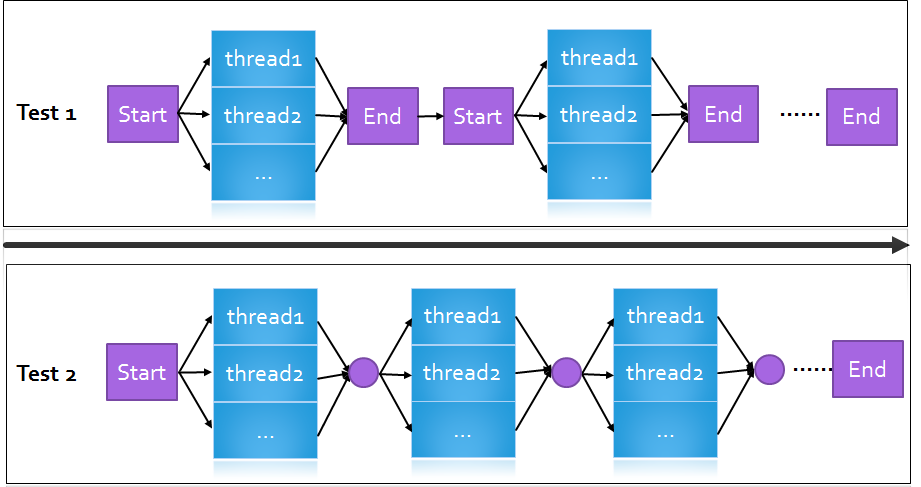
\includegraphics[width=0.7\textwidth] {images/quiesce_evaluation}
		\caption{omp\_quiesce evaluation}
		\label{omp:quiesce_evaluation}
	\end{figure}
	
	\begin{figure}
		\centering
		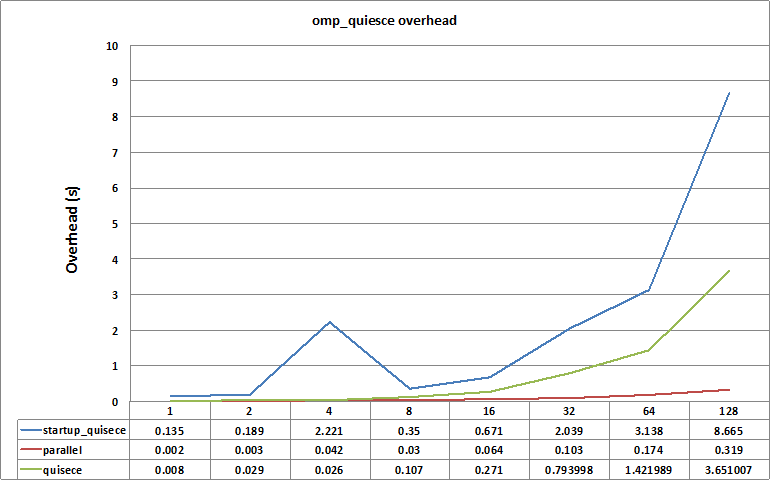
\includegraphics[width=0.7\textwidth] {images/quiesce_results}
		\caption{omp\_quiesce results}
		\label{omp:quiesce_results}
	\end{figure}
	
	
	\item void omp{\_}set{\_}wait{\_}policy(PASSIVE \textbar ACTIVE)
	
	We need to create two processes since each process will only maintain and share one thread pool. For those two process, each task is execute using 1s, and we need to create enough threads to make full use of the calculation power of one CPU. We tested it in three cases: passive, active, and quiesce/restart the runtime environment. Figure~\ref{omp:wait_policy_evaluation} shows the design of the evaluation.
	
	\begin{figure}
		\centering
		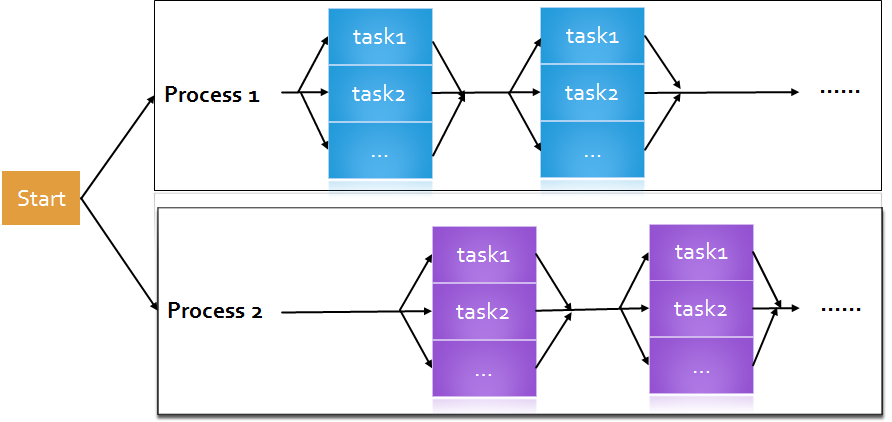
\includegraphics[width=0.7\textwidth] {images/wait_policy_evaluation}
		\caption{waiting policy evaluation}
		\label{omp:wait_policy_evaluation}
	\end{figure}
	
	As Figure~\ref{omp:wait_policy_results} below shows, there is no a big difference between the two behaviors. The reason is that the OpenMP uses only one global thread pool for all OpenMP threads created by multiple pthreads. So, the small difference comes from the time required to awake a sleeping thread. By doing this experiment, we have understand more about the way that OpenMP deals with the thread pool. 
	
	\begin{figure}
		\centering
		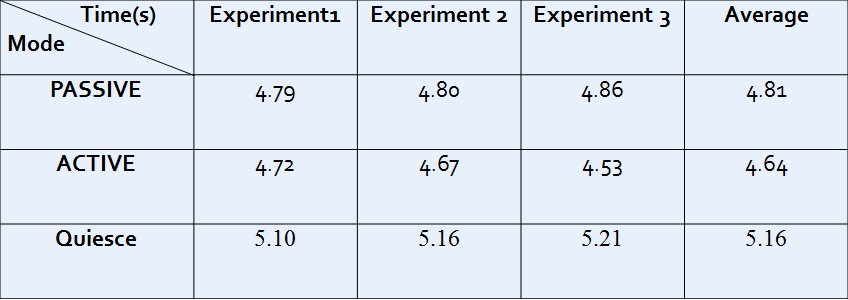
\includegraphics[width=0.7\textwidth] {images/wait_policy_results}
		\caption{Waiting Policy Results}
		\label{omp:wait_policy_results}
	\end{figure}
	
	
	\item int omp{\_}thread{\_}create()
	
	We compared this function with creating pthread to execute a list of tasks. So, for this function we have tested it in two different ways. Figure~\ref{omp:create_evaluation} shows the design of the evaluation. For the first way, we put different number of tasks in one parallel region, so that every “omp{\_}thread{\_}create()” or “pthread{\_}create()” function will be run in parallel. On the other hand, we use different iterations to execute the “omp{\_}thread{\_}create()” or “pthread{\_}create()” functions in sequence, and compare the running time. 
	
	\begin{figure}
		\centering
		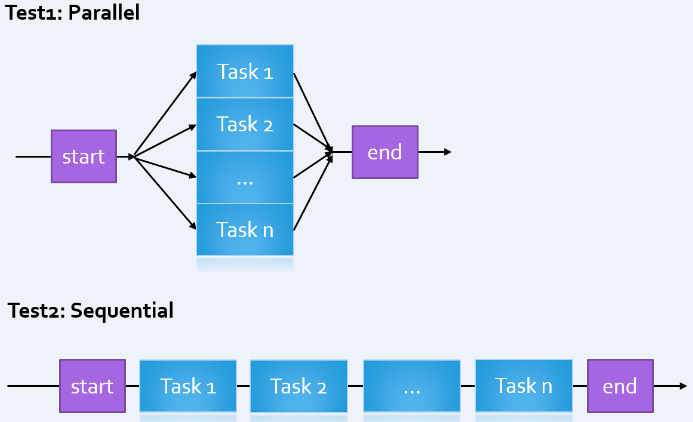
\includegraphics[width=0.7\textwidth] {images/create_evaluation}
		\caption{creating thread evaluation}
		\label{omp:create_evaluation}
	\end{figure}
	
	Figure~\ref{omp:create_results_parallel2} and Figure~\ref{omp:create_results_parallel} show the result of the first approach (execute in parallel). It clearly shows that there is almost no differences between them. This is might be because that we are doing it inside the parallel region.However, Figure~\ref{omp:create_results_sequence2} and Figure~\ref{omp:create_results_sequence} show the result of the second approach (execute in sequence). They show that omp{\_}thread{\_}create() gives a better performance that pthread{\_}create( ). So, it would be a good feature if the user can do this instead of creating another pthread.

% I do not think we need these.  The performance should be relatively obvious
% and in any case should not matter.  The purpose is to create an OS thread
% that the OpenMP runtime is aware of, and otherwise it should be the thinnest
% possible wrapper about the native OS thread library.
% Because of this, I do not see how omp_thread_create can be faster than
% pthread_create.
%                       - Jeff
\begin{comment}
	\begin{figure}
		\centering
		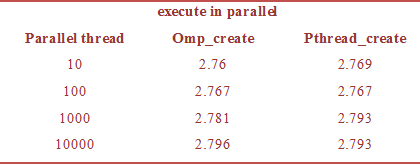
\includegraphics[width=0.7\textwidth] {images/create_results_parallel2}
		\caption{Results of omp\_thread\_create in parallel}
		\label{omp:create_results_parallel2}
	\end{figure}
	\begin{figure}
		\centering
		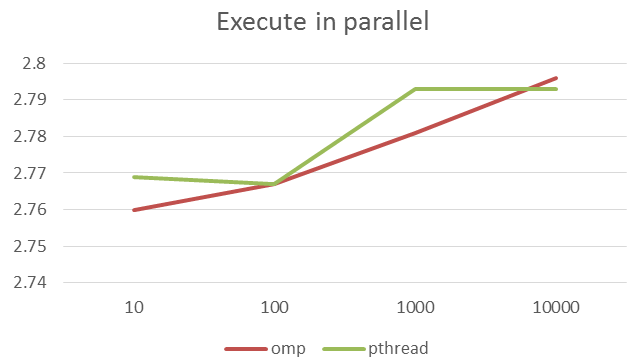
\includegraphics[width=0.7\textwidth] {images/create_results_parallel}
		\caption{Results of omp\_thread\_create in parallel}
		\label{omp:create_results_parallel}
	\end{figure}
	\begin{figure}
		\centering
		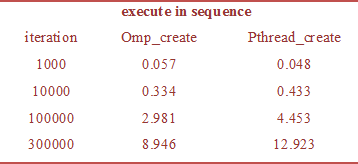
\includegraphics[width=0.7\textwidth] {images/create_results_sequence2}
		\caption{Results of omp\_thread\_create in sequence}
		\label{omp:create_results_sequence2}
	\end{figure}
	\begin{figure}
		\centering
		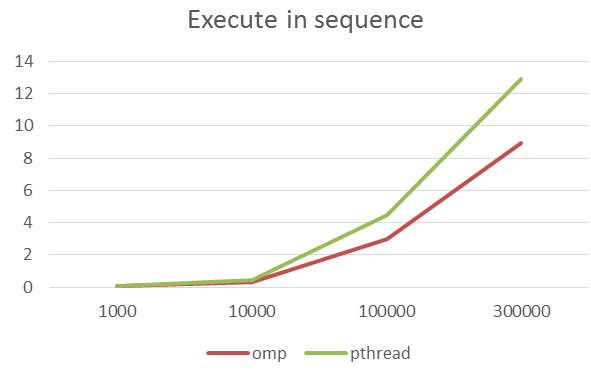
\includegraphics[width=0.7\textwidth] {images/create_results_sequence}
		\caption{Results of omp\_thread\_create in sequence}
		\label{omp:create_results_sequence}
	\end{figure}
\end{comment}

\end{enumerate}


